\chapter{Experimental Results}
In this chapter we will review the performance of our various algorithms on different types of worlds. These world showcase various scenarios that a motion planner may be presented with. 
\section{Worlds with Feasible Paths}
The following section is dedicated to worlds that are more common. These are worlds for which there exists a path from a start configuration to a goal configuration without needing to tolerate any collisions. We will look at two such examples: one that is mostly free space, and one that has many obstacles.

\subsection{Simple Minimal Obstacle World}
The first world of this type can be seen in Figure \ref{fig:common_world}.

\begin{figure}[h]
    \centering
    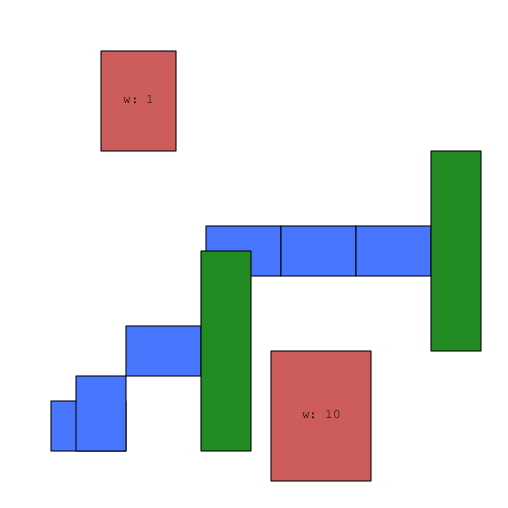
\includegraphics[width=0.5\textwidth]{feasible_world}
    \caption{Common Feasible World}
    \label{fig:feasible_world}
\end{figure}

\subsection{Cluttered World With Free Path}

\begin{figure}[h]
    \centering
    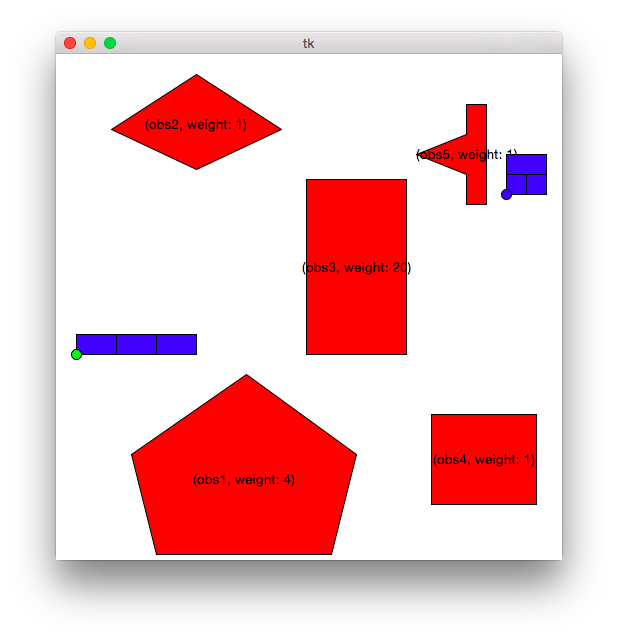
\includegraphics[width=0.5\textwidth]{many_obstacles_feasible_world}
    \caption{Cluttered Feasible World}
    \label{fig:many_obstacles_feasible_world}
\end{figure}

\section{Worlds with Nonexistent Collision Free Paths}

\subsection{Two Soda Can World}
\begin{figure}[h]
    \centering
    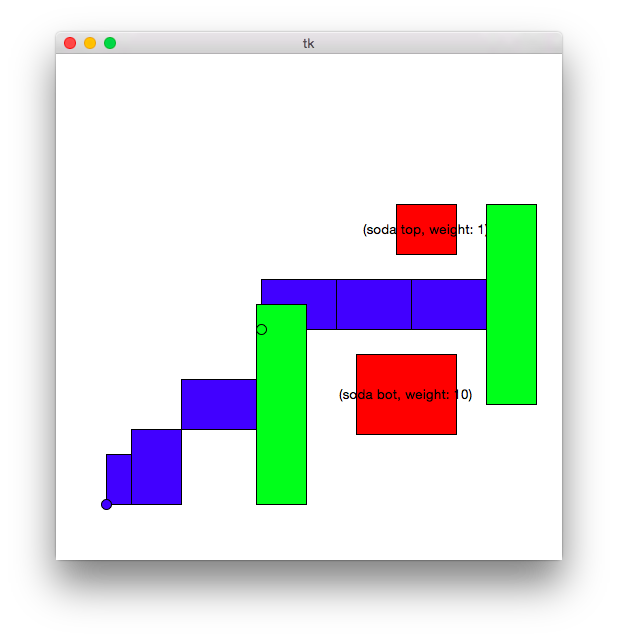
\includegraphics[width=0.5\textwidth]{two_soda_world}
    \caption{Two Box Unfeasible World}
    \label{fig:two_soda_world}
\end{figure}

\subsection{Almost Feasible Path World (MCR shines)}
\begin{figure}[h]
    \centering
    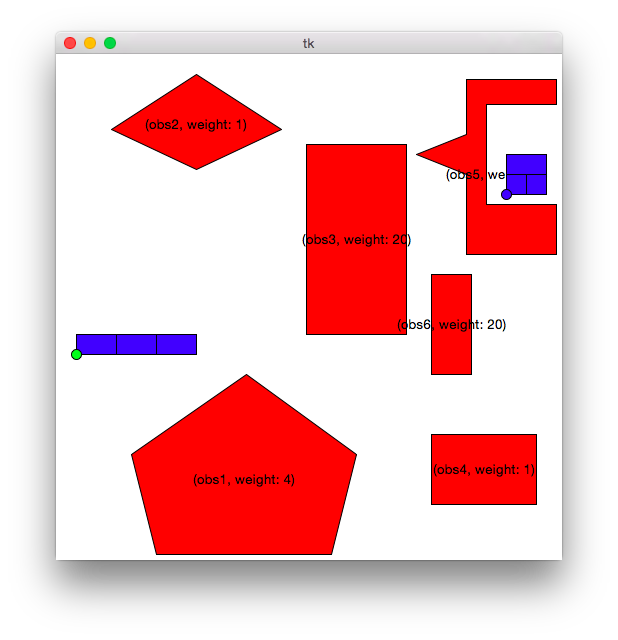
\includegraphics[width=0.5\textwidth]{many_obstacles_unfeasible_world}
    \caption{Nearly Feasible World}
    \label{fig:many_obstacles_unfeasible_world}
\end{figure}

\subsection{Cluttered World with Greedy Minimum Cover Path}
\begin{figure}[h]
    \centering
    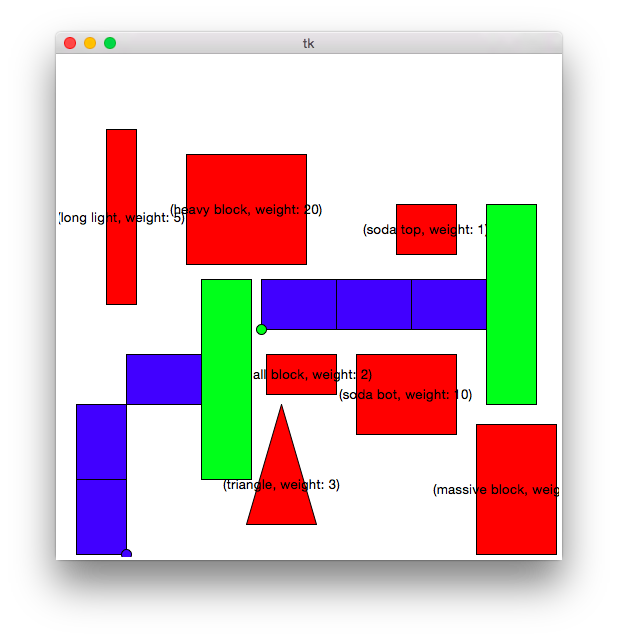
\includegraphics[width=0.5\textwidth]{cluttered_world}
    \caption{Cluttered World With Greedy Path of Minimum Cover}
    \label{fig:cluttered_world}
\end{figure}
\subsubsection{IterCount = 150}
\subsubsection{IterCount = 200}

\subsection{Cluttered World with Non-Greedy Minimum Cover Path}
\begin{figure}[h]
    \centering
    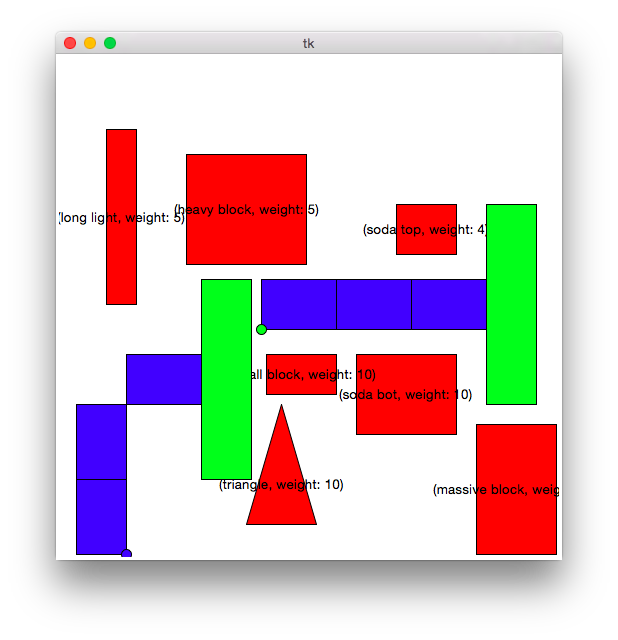
\includegraphics[width=0.5\textwidth]{top_light_cluttered_world}
    \caption{Cluttered World With Non-Greedy Path Of Minimum Cover}
    \label{fig:top_light_cluttered_world}
\end{figure}
\subsubsection{IterCount = 150}
\subsubsection{IterCount = 200}

\section{Discussion on Memory Factor Impact}
\subsection{Non Memory Factor Worlds Results Showing No Impact On Cover}
\subsection{Show Memory Factor Importance On Memory World}







